\documentclass[10pt]{report} 
\usepackage{amsmath, amsthm, amssymb, tikz, mathtools, hyperref,enumerate} 
\usepackage[margin=0.5in]{geometry} 
\newcommand{\scinot}[2]{#1\times 10^{#2}} 
\newcommand{\bra}[1]{\left<#1\right|} 
\newcommand{\ket}[1]{\left|#1\right>}
\newcommand{\dotp}[2]{\left<#1\left.\right|#2\right>}
\newcommand{\rd}[2]{\frac{d#1}{d#2}}
\newcommand{\pd}[2]{\frac{\partial #1}{\partial#2}}
\newcommand{\norm}[1]{\left|\left|#1\right|\right|}
\newcommand{\abs}[1]{\left|#1\right|}
\newcommand{\expvalue}[1]{\left<#1\right>}
\newcommand{\rtd}[2]{\frac{d^2#1}{d#2^2}}
\newcommand{\pvec}[1]{\vec{#1}^{\,\prime}}
\let\Re\undefined
\let\Im\undefined
\DeclareMathOperator{\Re}{Re}
\DeclareMathOperator{\Tr}{Tr}
\DeclareMathOperator{\Im}{Im}
\newcommand{\ptd}[2]{\frac{\partial^2 #1}{\partial#2^2}}
\usepackage[labelfont=bf, font=scriptsize]{caption}
\everymath{\displaystyle}
\begin{document}
\title{Astrophysique Stellaire\\ Amphi Cauchy M 1030-1200, 1330-1530\\ Fr\'ed\'eric Daigne, Roland Lehoucq CPHT-X}
\author{Yubo Su}
\date{}
\maketitle

\tableofcontents

\chapter{Id\'ees essentiel}

\begin{itemize}
    \item A l'angle d'une seconde, les deux jambes du triangle sont $1$UA et $1$pc.
    \item Equation de transfert $\rd{I_\nu}{s} = j_\nu - \alpha_\nu I_\nu$ ou avec $d\tau_\nu = \alpha_\nu ds$ on a $\rd{I_\nu}{\tau_\nu} = -I_\nu + S_\nu$. $j$ c'est la source et $I$ la luminosi\'e.
    \item Selon ci-dessus, \'epaisseur optique $\tau_\nu = \int \alpha_\nu ds$.
    \item $x = \frac{P_F}{mc} = \left( 3\pi^2 \right)^{1/3}\left( \frac{\hbar c}{mc^2} \right)n^{1/3}$. Si $x \ll 1$ on est non-relativiste, et si $x \gg 1$ on est ultra-relativiste.
    \item Le th\'eor\`eme du viriel $P = -\frac{E_g}{3V} = \frac{\alpha}{4\pi}\frac{GM^2}{R^4}$.
    \item La pression pour un gaz non-relativiste est $P = \frac{K}{m}n^{5/3}$ et pour un gaz ultra-relativiste $P = \frac{K}{m}n^{4/3}$. Aussi, pour les deux cas ce sont $P = \frac{2}{3}u, \frac{1}{3}u$ respectivement.
\end{itemize}
\chapter{Resum\'e du livre}

\section{Description des \'etoiles}

On mesure la distance des \'etoiles en \emph{parsec}, la distance ou la variation annuelle d'une \'etoile est une seconde d'arc. Il fait $1\mathrm{pc} = 206265\mathrm{ua}$ unit\'es astronomiques.

Les masse des \'etoiles sont mesurer en masse solaire $1 M_{\odot} = \scinot{1.989}{30}\mathrm{kg}$. On le d\'eduit pour les \'etoiles du systeme binaire en mesurant la p\'eriode de r\'evolution et le demi-grand axe $a$ de l'orbit, apr\`es qu'on peut calculer la masse par la trois\`eme loi de Kepler. 

On appelle la magnitude apparente la quantit\'e $m = -2.5\log \frac{F}{F_0}$ la luminosit\'e des \'etoiles. $F$ est le flux lumineux et $F_0$ est un flux de r\'ef\'erence quelconque. En prenant l'\'etoile V\'ega comme $F_0$, le Soleil a une magnitude apparente de $m=-26.7$ et les objets les plus faibles ont $m=31.0$. L'oeil nu ne peut pas voir plus faible que $m=6.0$.

Les \'etoiles rayonnent selon deux loi. La loi de Stefan $\phi = \sigma T^4$ donne l'intensit\'e du flux de l\'etoile. La loi de Wein $\lambda_0 T = 2898\mathrm{\mu m \cdot K}$ donne le maximum du flux comme fonction de la longeur d'onde.

Les \'etoiles se classifient par $7$ cat\'egories O B A F G K M en ordre de la temperature d\'ecroissant, chaque types comporte $10$ subdivisions num\'erot\'ees $0$ \`a $9$.

Si on place les \'etoiles sur une diagramme de la magnitude absolue $M$ en fonction de la couleur, on trouve qu'ils ne se distribuent pas n'importe comment mais de la forme d'un $\lambda$ tourn\'ee. Les deux groupes sont la s\'equence principale (qui forme une diagonale d\'ecroissant) et les [super-]g\'eantes au-dessus de cette s\'equence. On appelle ce diagramme le \emph{diagramme de Herzsprung-Russel}. 

L'int\'erieure des \'etoiles est rest\'ee longtemps une myst\`ere, mais r\'ecemment on a commenc\'e d'\'etudier les oscillations de la surface du Soleil avec les satellites comme Kepler. Ca nous donne des d\'etails de l'int\'erieure du Soleil.

\section{Formation des \'etoiles}

\subsection{Le milieu interstellaire}

On parle d'abord du milieu interstellaire, duquel toutes \'etoiles viennent. En premi\`ere approximation il s'agit de trois phase en \'equilibre, la phase froide, la phase chaude, et la phase tr\`es chaude. Le chauffage du mileu interstellaire est d\^u \`a l'irradiation par les \'etoiles, et le refroidissement \`a la conversion d'\'energie cin\'etique en photons. 

Soit $P_{eq}$ la pression o\`u les deux processus sont en \'equilibre, la stabilit\'e de l'\'equilibre entre les deux processus d\'epend $\rd{P_{eq}}{n}$. Si $\rd{P}{n} < 0$, alors \c{c}a veut dire que si on fait une petite perturbation $\delta n < 0$, $\delta P_{eq} > 0$ et on se trouve dans une r\'egion ou le chauffage domine. Ca augment encore $P_{eq}$ et on trouve que l'\'equilibre n'est pas stable par cet effet.

\subsection{Formation Stellaire}

Aux \'echelles astronomiques, la gravitation domine. Un corps de la densit\'e $\rho$ s'effond au temps caract\'eristique $\tau = \frac{1}{\sqrt{4\pi G\rho}}$. Si l'\'etoile ne s'effond pas, il faut qu'il y aie une force qui r\'eagit contre la force de gravitation; on sait que c'est la pression interne. On va analyser dans quelles conditions les \'etoiles forment.

Le temps caracteristique de la force de pression interne est donn\'e par $t_s = \frac{R}{c_s}$ o\`u $R$ est le rayon du syst\`eme et $c_s$ est la vitesse du son dans le milieu. Lorsque $\tau \gg \tau_s$ on trouve l'effondrement et lorsque $\tau_s \ll \tau$ on trouve que la pression r\'eagit plus vite que la gravitation et on ne trouve pas l'effondrement. Donc l'\'egalite $\tau_s = \tau$ d\'efinit une taille critique $R_c = \frac{c_s}{\sqrt{4\pi G\rho}}$ au-del\`a de laquelle l'effondrement peut avoir lieu.

Encore plus pr\'ecisement, on \'etudie l'effondrement par les lois de la dynamique des fluides. On commence avec un syst\`eme en \'equilibre et on le perturbe et calcule la stabilit\'e de cette perturbation. On trouve l\'equation qui s'agit de cette perturbation, qu'on prende comme une onde plane, est
\begin{align}
    \rtd{\delta_k}{t} + \left( c_s^2k^2 - 4\pi G\rho_0 \right)\delta_k &= 0
\end{align}

Lorsque $\left( c_s^2k^2 - 4\pi G\rho \right) > 0$ on trouve $\delta_k$ reste en forme de l'onde plane. Par contre si $\left( c_s^2k^2 - 4\pi G\rho \right)< 0$ on trouve $\delta_k$ prende la forme des exponentielles r\'eelles et la pertubation est donc instable. Comme \c{c}a on trouve la masse et la taille de Jeans, plus desquelles on trouve l'effondrement du milieu interstellair et la formation stellaire.
\chapter{14/09/14 --- Introduction, des petits trucs} 

On a besoin des telescopes de plus grande taille pour beaucoup de raisons: collecter plus de lumi\`ere, baisser la diffraction (les disques d'Airy, par l'\'equation $\theta = 1.22 \frac{\lambda}{D}$).  

Comment est-ce que la lumi\'ere est att\'enu\'e? Par l'\'equation
\begin{align}
    dI_\lambda = -\alpha_\lambda I_\lambda ds &= -\rho \kappa_\lambda I_\lambda ds
\end{align}
ou $\alpha_\lambda$ est le coefficient d'absorption et $\kappa_\lambda$ est l'opacit\'e. Deux proc\`ede contribuent \`a l'opacit\'e, l'absorption et la diffusion (ou le photon change sa direction). Soit donc $\tau_\lambda$ la ``optical depth''
\begin{align}
    \tau_\lambda = \int_C \alpha_\lambda ds
\end{align}

Les objects avec $\tau_\lambda \ll 1$ sont transparents, et lesquelles avec $\tau_\lambda \gg 1$ sont opaques.

On peut construire une quantit\'e luminosit\'e apparant $m = -2.5 \log_{10} \frac{E}{E_0}$ (souvent $E_0$ c'est la magnitude de l'\'etoile Vega). Par exemple, pour le Soleil $m = -26.7$, la lune $m = -12.9$, limite a l'\oe il nu $m = +6.0$.

A cause des perturbations atmospheriques les images des telescopes ne sont pas bien; on peut faire des ``adaptive optics'' pour l'am\'eliorer. On deforme les miroirs en temps r\'eels pour annuler ces perturbations. On utilise un laser pour cr\'eer une \'etoile artificielle dont on peut determiner les d\'eformations de l'atmosphere en temps r\'eels.

A cause du mouvement de la Terre les \'etoiles bougent au ciel; ce mouvement angulaire peut \^etre m\'esurer, et on l'appelle le ``parallaxe.''

Il faut observer les m\^emes galaxies en beaucoup de longeur d'ondes. Par exemple, quand on regarde la galaxie Androm\`ede en infra-rouge, rayons X, et la lumi\'ere visible, on voit beaucoup de differences!

La densit\'e spectrale des photons est ecrit comme
\begin{align}
    n(\nu) d\nu = 2\frac{4\pi \nu^2 d\nu}{c^3}\frac{1}{\exp\left( h\nu/kT \right) - 1}
\end{align}

La derni\'ere partie est la distribution de Bose, parce que les photons sont des bosons. La deuxi\'eme partie est la densit\'ee des \'etats $\frac{4\pi \rho^2 d\rho}{h^3}$ dans l'espace de phase, ou $\rho = \frac{h\nu}{c}$. Enfin le $2$ c'est parce que les photons ont $2$ polarizations.

On peut aussi calculer la densit\'e d'energie $u = \int\limits_{0}^{\infty}h\nu \times n(\nu) \;d\nu \propto T^4$. 

Selon la spectre d'absorption des \'etoiles on peut d\'eduire les \'el\'ements chimiques qui sont presentes dans les \'etoiles. En comparisant les lignes d'absorption et la spectre d'emission (dont on peut d\'eduire la temperature de l'\'etoile) on peut determiner quels \'el\'ement sont pr\'esents dans les \'etoiles de quelle temperature.

Si on ecrit l'\'energie d'une syst\`eme des $N$ protons et \'electrons, on a (si on \'ecrit $d$ pour la distance characteristique entre un proton et un \'electron)
\begin{align}
    E(N,d) = N\left( \frac{p_p^2}{2m_p} + \frac{p_e^2}{2m_e} - \frac{e^2}{d} \right)
\end{align}

Mais nous savons que $p_p \sim p_e \sim \frac{\hbar}{d}$, et parce que $m_e \ll m_p$ on supprime la premi\'ere partie de l'expression et on a
\begin{align}
    E(N,d) = N\left( \frac{1}{2m_e}\left( \frac{\hbar}{d} \right)^2 - \frac{e^2}{d} \right)
\end{align}

Si on cherche le minimum de cette \'en\'ergie, nous trouvons que $d = a_0$ le rayon Bohr! Aussi, le minimum $E_0(N,d) = -N\left( \varepsilon_0 = 13.6\mathrm{eV} \right)$ et donc on a tous les resultats de m\'ecaniques quantiques.

On peut faire les m\^emes calcul pour l'\'en\'ergie gravitationelle et on trouve que $E_0(N) = -N^{7/3}\left( \frac{Gm_p^2}{e^2} \right)^2 \varepsilon_0$, et donc nous trovons la limite o\`u la force gravitationelle peut dominer la force electrostatique, $N \sim 10^{54}$.
\chapter{14/09/14 --- PC1, Probl\`emes concernant la radiation}

\begin{enumerate}[1)]
    \item Bilan Radiatif du Corps Humain
        \begin{enumerate}[i)]
            \item \emph{Faites votre bilan radiatif dans une pi\`ece chauf\'ee \`a $20^\circ$C. Vous supposerez que votre corps rayonne comme un corps noir dont la temp\'erature est celle de la peau, soit environ $27^\circ$C.} 
                
                On calcule la difference du flux entre le corps et la pi\`ece, et donc $\Delta \mathcal{P} = \sigma\left( (293^\circ \mathrm{K})^4 - (300^\circ\mathrm{K})^4 \right) = \boxed{-41.4\mathrm{W\;m^{-2}}}$. 
            \item \emph{Quelle est la puissance nette que vous rayonnez?}
                
                Si on fait l'assumption que l'aire du corps est $\sim 2 \mathrm{m^2}$ on arrive a $\boxed{\Delta P \approx -80 W}$.
        \end{enumerate}
    \item Temp\'erature d'\'equilibre de la terre et des plat\`etes.
        \begin{enumerate}[i)]
            \item \emph{En ignorant l'atmospher\`ere de la Terre ecrire la relation liant la luminosit\'e Soleil $L_{\odot}$ \`a sa temp'\'erature $T_{\odot}$ et \`a son rayon $R_\odot$. En d\'eduire le flux re\c{c}u par la Terre situ\'ee \`a la distance $D$.}

                Nous savons que $\mathcal{P}_\odot = \sigma T_\odot^4$ et donc $L_\odot = \mathcal{P}_\odot \cdot (4\pi R_{\odot}^2) = \boxed{4\pi R_{\odot}^2 \sigma T_{\odot}^4}$. Donc, si on appelle $D = 1\mathrm{UA}$ (unit\'e astronomique) on sait que le flux re\c{c}u par la Terre est $\Phi_E = \frac{L_{\odot}}{4\pi D^2} = \sigma T_{\odot}^4 \frac{R_{\odot}^2}{D^2}$\footnote{On appelle la taille angulaire du Soleil $\alpha$ le ``apparent radius.'' C'est tr\`es naturelle de definir \c{c}a parce que \c{c}a appara\^it dans l'\'equation.}.
            \item \emph{La Terre r\'efl\'echit la fraction $\alpha = 0.3$ du rayonnement solaire incident (on appelle $\alpha$ l'alb\'edo). Trouver la relation qui, \`a l'\'equilibre, lie la temp\'erature moyenne de la Terre $T_E$ \`a celle du Soleil.}

                On commence en \'ecrivant $P_E = 4\pi R_E^2 \sigma T_E^4$ la puissance de radiation de la Terre. Aussi, on sait que l'aire de la Terre qui re\c{c}oit de la radiation du Soleil est $\pi R_E^2$ et donc $P_{abs} = (1-\alpha)\pi R_E^2 \Phi_E$. On les met \'egales comme
                \begin{align}
                    4\pi R_E^2 \sigma T_E^4 &= (1-\alpha)\pi R_E^2 \Phi_E\\
                    T_E^4 &= \frac{(1-\alpha)\pi T_{\odot}^4\frac{R_{\odot}^2}{D^2}}{4\pi}\\
                    T_E &\approx 254^\circ \mathrm{K}
                \end{align}

                C'est moins que la vrai temp\'erature $288^\circ \mathrm{K}$.

            \item \emph{Dotons maintenant la Terre d'une atmosph\`ere transparente \`a la lumi\`ere visible mais opaque \`a la lumi\`ere infrarouge. Ecrire le bilan radiatif du sys\`eme Terre+atpmosph\`ere et en d\'eduire la nouvelle temp\'erature d'\'equilibre de la plan\`ete.}

                On a maintenant deux \'equilibre \`a calculer. Pour l'atmosphere et la Terre respectivement
                \begin{align}
                    4\pi R_E^2\sigma T_E^4 &= 2\times 4\pi R_E^2 \sigma T_{atm}^4 & (1-\alpha)\pi R_E^2 \Phi_E + 4\pi R_E^2 \sigma T_{atm}^4 &= 4\pi R_E^2 \sigma T_E^4\label{15.9.eq1}\\
                    &&(1-\alpha)\pi R_E^2 \Phi_E + \frac{4\pi R_E^2\sigma T_E^4}{2} &= 4\pi R_E^2 \sigma T_E^4\\
                    &&2\pi R_E^2 \sigma T_E^4 &= (1-\alpha)\pi R_E^2 \Phi_E\\
                    &&T_E^4 &= \frac{(1-\alpha) T_{\odot}^4\frac{R_{\odot}^2}{D^2}}{2}\\
                    &&T_E &\approx 302
                \end{align}
                ($2\times$ \`a droit de l'\'equation \eqref{15.9.eq1} parce qu'il rayonne dans deux directions, \`a la Terre et au Soleil)
        \end{enumerate}
    \item Estimation de la distance de Sirius par la m\'ethode de Gregory
        \begin{enumerate}[i)]
            \item \emph{Exprimez le flux que Jupiter re\c{c}oit du Soleil. En d\'eduire la puissance totale que Jupiter \'e\'emet vers l'espace en supposant que la plan\`ete est parfaitement r\'efl\'echissante}

                On peut simplement prendre la resultat de la probl\`eme pr\'ec\'edant, $P_J = \pi R_J^2\frac{L_{\odot}}{4\pi D_J^2}$.
            \item \emph{Exprimez maintenant le flux lumineux que la Terre re\c{c}oit de Jupiter. En d\'eduire une \'egalit\'e qui vous permettra d'obtenir la distance de Sirius.}

                Soit $D_{EJ}$ la distance entre la Terre et Jupiter. Donc le flux que la Terre re\c{c}oit de Jupiter est
                \begin{align}
                    \Phi_{EJ} &= P_J \frac{R_E^2}{4D_{EJ}^2}\\
                    &= R_J^2\frac{L_{\odot}}{4 D_J^2}\frac{R_E^2}{4D_{EJ}^2}\\
                    &= \pi R_{\odot}^2 \sigma T_{\odot}^4\frac{R_J^2}{ D_J^2}\frac{R_E^2}{4D_{EJ}^2}
                \end{align}

                Maintenant en assumant que la luminosit\'e de Sirius et la m\^eme que le Soleil, on peut mettre \'egal les deux expressions
                \begin{align}
                    \sigma T_{\odot}^4 \frac{R_{\odot}^2}{D_S^2}&= \pi R_{\odot}^2 \sigma T_{\odot}^4\frac{R_J^2}{ D_J^2}\frac{R_E^2}{4D_{EJ}^2}
                \end{align}

                Je n'ai pas fini cette \'exercise mais la r\'eponse est $83190 \mathrm{UA}$.
        \end{enumerate}
    \item Performance de d\'etection selon la taille du collecteur de lumi\`ere. La magnitude limite visible \`a l'oeil nu est $m_0 = 6$.
        \begin{enumerate}[i)]
            \item \emph{Rappelez que $m = -2.5 \log_{10} \frac{\Phi}{\Phi_0}$. Calculez le flux re\c{c}u d'une \'etoile de la magnitude $m_0$ sachant que la magnitude apparente du Soleil est de $m_{\odot} = -26.72$.}

                on sait que $m_0 - m_{\odot} = -2.5\log_{10}\frac{\Phi_0}{\Phi_{\odot}} = 6 + 26.72 = 32.72$. Donc on \'ecrit
                \begin{align}
                    \log_{10}\frac{\Phi_{\odot}}{\Phi_0} &= 13.1\\
                    \Phi_0 &= \frac{\Phi_{\odot}}{10^{13.1}}
                \end{align}
                
                Si on utilise $\Phi_{\odot} = \Phi_E = \frac{L_{\odot}}{4\pi D^2} \approx 1358.12 \mathrm{W\; m^{-2}}$ on voit que $\Phi_0 \approx \scinot{1.08}{-10}\mathrm{W\;m^{-2}}$.
            \item \emph{Quelle est la puissance nette que re\c{c}oit l'oeil?}

                La diam\`etre de la pupille est d'environ $6\mathrm{mm} = \scinot{6}{-3}\mathrm{m}$ et donc
                \begin{align}
                    P_0 &= \scinot{1.08}{-10} \left( \scinot{6}{-3} \right)^2 \pi\\
                    &= \scinot{1.22}{-14}\mathrm{W}
                \end{align}
            \item \emph{En supposant que le seul param\`etre influant $m_0$ est le diam\`etre du collecteur, exprimer $m_0(D)$ en fonction de ce diam\`etre $D$.}

                Notez que $m_0(D) = -2.5\log_{10}\frac{P_0/\pi D^2}{\Phi_0}$. Si on l'\'exprime en fonction de $m_0^{oeil}$ on obtiens
                \begin{align}
                    m_0(D) &= -2.5\left( \log_{10}\frac{P_0/\pi D^2}{P_0/\pi d_{oeil}^2}\right)  + m_0^{oeil}\\
                    &= 5\log_{10}\frac{D}{d_{oeil}} + m_0^{oeil}
                \end{align}
        \end{enumerate}
\end{enumerate}
\chapter{22/09/14 --- Le milieu interstellaire, La formation des etoiles}

\section{Le milieu interstellaire}

Dans l'atmosph\`ere, la densit\'e des particules est $10^{19}$ (``dix puissance dix-neuf''), et laquelle entre les etoiles est $10^{-3}-10^{6}$. On dit $C_{IV} = C^{3+}, O_{III} = O^{2+}$. Parce qu'il y a beaucoup de rayons jet\'e par les Soleil qui interagit avec le milieu interstellaire, il y a beaucoup de phenom\`ene qu'on peut d\'ecrire; on va les parler tout simplement!

Il y a trois cat\'egories de temperature dans le milieu interstellaire
\begin{itemize}
    \item Froid --- Neutre, beaucoup de molecules et de poussi\'ere (\emph{dust}), temperature $10-100$K.
    \item Chaud --- Gaz ionis\'e ou gaz neutre, des nuages de mati\'ere, temperature $8000$K.
    \item Br\^ulant --- Tr\'es ionis\'e, produit par les supernovae, temperature $10^6$K.
\end{itemize}

A l'\'equilibre de pression, le milieu interstellaire froid et au centre, ensuite lequel chaud neutre, ensuit lequel chaud ionis\'e, et finalement lequel br\^ulant. En realit\'e c'est beaucoup plus complexe! Il y a beaucoup d'\'equilibres qui se battent; aucun ne domine! Par exemple, a l'\'equilibre de pression on a des chauffages et des refroidissements entre les diff\'erent mileus interstellaires. Quelques m\'ecanisms:
\begin{itemize}
    \item Chauffage --- absorption des photons UV, ionisation
    \item Refroidissement $T < 10000$K --- excitation de $C_{II}$ par des collisions avec des electrons et \'emission des photons
    \item Refroidissement $T > 10000$K --- excitation ou ionisation de $H_{I}$ par des collisions avec des electrons et \'emission des Lyman $\alpha$
\end{itemize}

Nous commen\c{c}ons la solution avec l'\'equation du transf\`ere radiatif
\begin{align}
    \rd{I_\nu}{x} &= -\alpha_\nu I_\nu + j_\nu
\end{align}

On change les variables et appelle  $S_\nu \equiv \frac{j_\nu}{\alpha_\nu}$ la fonction de source. A l'\'equilibre, la source est la fonction de Planck
\begin{align}
    \rd{I_\nu}{\tau_\nu} &= -I_\nu + S_\nu\\
    I_\nu(\tau_\nu) &= I_\nu(0)e^{-\tau_\nu} + \int\limits_{0}^{\tau_\nu}S_\nu(\tau')e^{-(\tau_\nu -\tau')}\;d\tau'
\end{align}

La premi\`ere terme est la source d'arri\`ere-plan qui n'est pas absorb\'ee, et la deuxi\`eme est l'\'emission et l'adsorption dans la nuage de la mati\`ere. En 1D, la solution est $I_\nu(\tau_\nu) = I_\nu(0) e^{-\tau_\nu} + S_\nu\left( 1 - e^{-\tau_\nu} \right)$.

Le rayonnement de CMB est presque exactement un ``blackbody'' de $2.725$K. 

Le milieu interstellaire est adiaphane au rayonnement UV, mais il est diaphane au rayonnement infrarouge. On ne peut pas observer les rayons gamma, et les rayons-X sont tr\`es difficile \`a r\'efl\'echir.

\section{La formation des \'etoiles}

Consid\`erer une nuage sph\`erique du masse $M$; une particule sur la surface tombe par l'\'equation $\ddot{r} = -\frac{GM}{r^2}$, et apr\`es trouver la solution on trouve qu'il tombe d'un ``timescale'' $\tau \simeq \frac{1}{\sqrt{4\pi G\rho}}$.

Il y a trois sources de pression internelle: temperature, magnetisme, et turbulence. Toutes les trois d\'ecroissent comme $M^{-1}$ ou $M^{-2}$, et donc plus lourd que l'\'etoile, moins fort les autres sources de pression. C'est naturel qu'il y a une mass maximume ou $\rho$ la densit\'e accro\^it exponentiellement.. En faisant beaucoup des assumptions on peut calculer cette masse, la masse de Jean.

Cette masse est $\sim10^{8}M_{\odot}$. Si on est plus lourd que \c{c}a, on collapse. Pendant la collapse, la masse de Jean decro\^it, et a cause de \c{c}a beaucoup des petites pi\`eces forment. Eventuellement, la nuage devient adiaphane \`a la radiation, et la syst\`eme devient ferm\'ee.
\chapter{22/09/14 --- PC2}

Noter qu'un parsec est la distance ou la parallax est un arcsecond, $\approx 206265 \mathrm{UA} \approx \scinot{3}{18}\mathrm{cm} \approx 3.26\mathrm{LY}$. Noter qu'un arcsecond est $\frac{1}{60}$ d'une minute qui est $\frac{1}{60}$ d'un degr\'ee.

\section{Assombrissement centre-bord, ``limb darkening''}

\begin{enumerate}[i)]
    \item \emph{On construit un premier mod\`ele simple pour expliquer cette ph\'enom\`ene: l'\'emission est en partie absorb\'ee par une atmosph\`ere d'\'epaisseur optique $\tau_\nu$ dans la direction radiale. Calculer $I(\theta)$ en assumant que le Soleil rayonn \`a une intensit\'e $I_0$.}

        A une angle $\theta$ de la ligne de vis\'ee la rayon traverse une distance augment\'ee par $\frac{1}{\cos\theta}$ dans l'atmosph\`ere, et donc c'est une diminution exponentielle, comme $I = I_0 e^{-\frac{\tau_\nu}{\cos\theta}}$. C'est \'evidement pas correcte; c'est pas la diminution qu'on observe.

    \item \emph{On raffine le mod\`ele pr\'ec\'edent en consid\'erant le milieu solaire comme un milieu continu dans lequel \'emission et absorption ont \`a la fois lieu. Qualitativement, est-ce que \c{c}a r\'esout la probl\`eme?}

        Il faut au premier noter qu'il y a une limite de profondeur optique. Donc, la plus $\theta$, la plus froide est la limite de la profondeur optique, et on retrouve l'assombrissement centre-bord.

    \item \emph{Ecrire l'\'equation du transfert du rayonnement pour $I(\tau_\nu, \cos\theta)$. On d\'efinit $d\tau_\nu = -\alpha_\nu dr$, soit $dr$ la \'epaisseur de la couche infinit\'esimale. Noter que $s$ et la direction radiale et $r$ est la direction vers l'observateur.}

        On commence avec 
        \begin{align}
            dI_\nu &= -\alpha_\nu I_\nu ds + j_\nu ds\\
            &= -\alpha_\nu ds\left( I_\nu - S_\nu \right)\\
            &= -\alpha_\nu \frac{dr}{\cos\theta}\left( I_\nu - S_\nu \right)\\
        \end{align}
        ou on utilise souvent $S_\nu = B_\nu(T)$ la radiation d'un corps noir. On continue en ecrivant une int\'egrale
        \begin{align}
            \rd{I_\nu}{\tau_\nu} &= \frac{I_\nu}{\cos\theta} - \frac{S_\nu}{\cos\theta}
        \end{align}
        
        On utilise un ``integrating factor'' $e^{-\frac{\tau_\nu}{\cos\theta}}$ et obtient
        \begin{align}
            \int\limits_{\tau_\nu}^{\infty}\rd{}{\tau}\left( I_\nu e^{-\tau'/\cos\theta} \right)\;d\tau &= \int\limits_{\tau_\nu}^{\infty}-\frac{S_\nu(\tau')}{\cos\theta}e^{-\tau'/\cos\theta}\;d\tau'\\
            I_\nu &= \int\limits_{\tau_\nu}^{\infty}\frac{S_\nu(\tau')}{\cos\theta}e^{(\tau_\nu - \tau')/\cos\theta}\;d\tau'
        \end{align}

        On voit que plus profonds que sauf une profondeur mince sur la surface le Soleil est adiaphane.

    \item \emph{On veut utiliser $S_\nu = B_\nu(T)$, mais on a une fonction de $\tau$! D'apr\`es Eddington, on prend $S_\nu = a_\nu + b_\nu \tau_\nu$. Calculer $I_\nu(0,\cos\theta)$}

        \begin{align}
            I_\nu(0,\cos\theta) &= \frac{1}{\cos\theta}\int\limits_0^{\infty}\left( a_\nu + b_\nu \tau' \right)e^{ - \tau'/\cos\theta}\;d\tau'\\
            &=\int\limits_{0}^{\infty}\left( a_\nu + b_\nu u \cos\theta \right)e^{-u}\;du\\
            &= a_\nu + b_\nu\cos\theta
        \end{align}

    \item \emph{Il est insens\'e de parler de la ``temperature'' du Soleil; il est seulement possible de definer une ``temperature effective'' \`a laquelle un corps noir aura la m\^eme flux spectral que le Soleil. On d\'eduit le flux spectral du Soleil $F_\nu$ et compare \`a la valeur pour les corps noir $F_\nu = \pi B_\nu(T_{eff})$.}

        \begin{align}
            F_\nu &= \int\limits_{0}^{\pi/2}\left( a_\nu + b_\nu\cos\theta \right)\cos\theta 2\pi\;\left( -d(\cos\theta) \right)\\
            &= 2\pi \int\limits_{0}^{1}\left( a_\nu + b_\nu u \right)u\;du\\
            &=\pi\left( a_\nu + \frac{2}{3}b_\nu \right) = \pi S_\nu\left( \frac{2}{3} \right)
        \end{align}
        et donc l'\'epaisseur optique du Soleil est $\tau = \frac{2}{3}$. 

        Ca montre que l'assombrissement centre-bord du Soleil \`a $\tau_\nu = 0$ est le m\^eme qu'un corps noir avec $\tau = \frac{2}{3}$. 

    \item Il faut noter que $I_\nu \sim \frac{2}{3} + \cos \theta$ est tr\`es proche aux don\'ees vraies.
\end{enumerate}

\section{Sph\`ere de Str\"omgren}

On mod\'elise la n\'ebuleuse de la Rosette comme une sph\`ere d'hydrog\`ene ionis\'e. Il y a une jeune \'etoile au centre qui \'emet $S_*$ photons par seconde, qui ionisent l'hydrog\`ene selon $H + h\nu \to p + e$. Soit $n_H, n_p, n_e$ les densit\'es volumetriques.

\begin{enumerate}[i)]
    \item \emph{A partir de la conservation de la mati\`ere et de la charge, donner deux relations entre $n_H, n_p, n_e$.} $n_p = n_e$ et $n_0 = n_p + n_H$ est constante.

    \item \emph{Ecrire l'\'evolution de la densit\'e d'hydrog\`ene neutre dans un volume de gaz situ\'e \`a la distance $r$ de l'\'etoile.}

        On commence avec $\rd{n_H}{t} = -\sigma_0n_HJ + \beta n_pn_e$ avec $J$ le flux des photons et $\beta$ la probabilit\'e de recombinaison. On sait que $J = \frac{S_*}{4\pi r^2}$.

        A l'\'equilibrium $\sigma_0 n_H \frac{S_*}{4\pi r^2} = \beta n_pn_e$. On appelle $n_0 = n_H + n_p = n_H + n_e, x = \frac{n_H}{n_0}$ et alors
        \begin{align}
            \sigma_0 n_0 x \frac{S_*}{4\pi r^2} &= \beta n_p^2\\
            &= \beta \left( n_0 - n_H \right)^2\\
            &= \beta n_0^2 \left( 1 - x \right)^2
        \end{align}

        Comme \c{c}a on peut calculer $x$. 
    \item \emph{Calculer la taille ou l'ionisation et la recombinaison sont \'equilibr\'ees.}
        
        On voit que les echelles de temps pour l'ionisation et la recombinaison sont $\frac{1}{\sigma_0J}, \frac{1}{\beta n_e}$ respectivement. Car $J \sim r^{-2}$, on peut les mettre \'egals et obtenir la valeur de $R_S$ ou l'ionisation et la recombinaison proc\'edent \`a la m\^eme taux; on appelle $R_S$ le rayon de Str\"omgren. A $r < R_S$ on voit que l'hydrog\`ene est pour la plupart ionis\'ee, et \`a $r > R_S$ on obtient l'hydrog\`ene neutrel.

        A $R_s$ on doit aussi avoir $S_* = \frac{4}{3}\beta n_en_p \pi R_s^3$ car on doit recombiner la m\^eme nombre des hydrog\`enes qu'on detruit.

    \item \emph{On s'interesse \`a la propagation d'ionisation. Suppose qu'on a une \'etoile au centre d'une sph\`ere pleine des hydrog\`enes neutres. Calculer $R(t)$, le rayon du sph\'ere d'ionisation.}

        Pendant un temps $dt$ on n'a que $S_* dt$ photon, et il faut ioniser $4\pi r_i^2 dR n_0$ molecules d'hydrog\'ene. Donc, sans recombinaison on a $R(t) = \left(\frac{3}{4\pi} \frac{S_*t}{n_0}\right)^{\frac{1}{3}}$. 

    \item \emph{Et avec la recombinaison?} On a simplement une \'equation differente $S_* dt = 4\pi R^2 dR n_0 + \beta n_en_p \frac{4}{3}\pi R^3(t) dt$.
\end{enumerate}
\chapter{29/09/14 --- La stabilit\'e des \'etoiles.}

Toutes les choses qui sont chaud brillent; les humains brillent \`a l'infrarouge, plus precisement \`a longeur d'onde 10$\mu$m. 

\section{Qu'est-ce que c'est une \'etoile?}

Que veut dire une \'etoile? C'est une grande boule de gaz, avec une mass mini et maxi qu'on peut calculer. La composition (par masse) est $\sim 73,5\%$ hydrog\`ene, $24,9\%$ h\'elium et $1,6\%$ les autre (comme carbon et fer).

On peut cr\'eer une diagramme de luminosit\'e versus l'inverse de la temperature, qui s'appelle une diagramme de \emph{Hertzsprung-Russel}. Rappeler que $L = 4\pi R^2 \sigma T^4$. Sur cette diagram, il y a la s\'equence principale dans laquelle il y a beacuoup des \'etoiles, mais il y a aussi des groupes des naines blanches, et les differents types de g\'eants.

\section{Th\'eor\`eme du viriel}

Pour determiner la structure des \'etoiles on commence en prenant les \'etoiles comme spheriques. C'est pas toujours le cas, par exemple Achernar qui tourne tr\`es vite ($\sim 225\mathrm{ km/s}$). Mais si on assume la sph\`ere on obtient que
\begin{align}
    g(r) &= \frac{GM(r)}{r^2} & dM &= 4\pi r^2 dr \rho(r)
\end{align}
\`a cause du gravit\'e. Aussi, la difference de pression doit balancer le poids, comme
\begin{align}
    \rd{P}{r} &= -\rho(r) g(r)
\end{align}

Si la pression dispara\^it, l'\'etoile va s'effondrer! On peut calculer l'\'echelle de temps que cette effondrement va prendre par $\rtd{r}{t} = -\frac{GM}{r^2} = -\frac{G}{r^2}\frac{4}{3}\pi r_0^3 \bar{\rho}$ et on obtient que l'\'echelle c'est $\tau_{eff} \sim \sqrt{\frac{3}{8\pi G\bar{\rho}}}$. 

La th\'eor\`eme du viriel (orth?) est trouv\'e comme
\begin{align}
    \rd{P}{r} &= -\rho g\\
    \frac{4}{3}\pi r^3 dr \rd{P}{r} &= - \frac{r}{3}\rho \frac{GM}{r^2} \underbrace{\rho 4\pi r^2 dr}{dM}\\
    \int\limits_{0}^{R_*}V\;dP &= \int\limits_{0}^{R_*}\frac{1}{3}\left( -\frac{GM}{r} \right)\;dM\\
    3PV &= -U_G
\end{align}

Si on assume un gaz parfait on obtient $2U + U_G = 0$ et donc l'\'energie totale $E = U + U_G = -U = \frac{U_G}{2}$. Pour une sph\`ere homog\'ene $U_G = -\frac{3}{5} \frac{GM^2}{R}$. 

Parce que $U_G < 0$ quand l'\'etoile rayonne d'\'energie le rayon diminue (pour diminuer l'\'energie).

On dit $\tau = \frac{U_G}{L_*}$ le temps characteristique d'une \'etoile qui rayonne \`a luminosit\'e $L_*$. Pour le Soleil, $\tau \sim 10^6$ ans, mais on a d\'ej\'a $\sim10^9$ ans! Comment est-ce que c'est possible? On a besoin de plus d'\'energie, et la seule source possible c'est l'\'energie nucl\'eaire.

\section{Mod\`ele stellaire}

On a maintenant $3$ \'equations et $4$ inconnu
\begin{align}
    \rd{P}{r} &= -\rho(r) g(r) & g(r) &= \frac{GM(r)}{r^2} & dM &= 4\pi r^2 dr \rho(r)
\end{align}

Si on veut utiiser un gaz, on a une autre \'equation, l'\'equation d'\'etat, mais aussi un autre inconnu la temperature.

On peut assumer une mod\`ele de gaz ``polytrope,'' $P = K\rho^{1 + \frac{1}{n}} = K\rho^{\gamma}$. Si on continue avec $\rho = \rho_c \phi^n, P = K\rho_c \phi^{n+1}$ (noter que $\rho_c$ c'est la densit\'e au centre) on a l'\'equation Lane-Emden
\begin{align}
    \frac{1}{u^2}\rd{}{u}\left( u^2\rd{\phi}{u} \right) &= -\phi^n
\end{align}
avec $u = \frac{r}{\lambda}, \lambda^2 = \frac{(n+1)K\rho_c^{\frac{1}{n} - 1}}{4\pi G}$. Les BC sont $\phi(0) = 1$ et $\rd{P}{r} = \rd{\phi}{u}(0) = 0$. 

Il y a quelques solutions, mais si $n \geq 5$, $\phi(u)$ n'a pas des z\'eros ($\forall u, \phi(u) \neq 0$). Les propri\'et\'e de l'\'etoile sont donc
\begin{itemize}
    \item Rayon --- $\phi(u) = 0$ signifie le rayon d'\'etoile, et donc $R \to \infty$ si $n \geq 5$.
    \item Masse --- $M = 4\pi \lambda^3 \rho_c \left( -u^2 \rd{\phi}{u} \right) \propto \rho_c^{\frac{3-n}{2n}}$
\end{itemize}

On peut calculer beaucoup plus, comme densit\'e, pression au centre, $U_{g}$, temperature au centre. D'apr\`es toutes ces calculs on peut r\'epondre \`a la question ``est-ce que la production d'\'energie nucl\'eaire et favorable?'' mais on ne fait pas \c{c}a au moment.

\section{H\'elios\'eismologie et astros\'eismologie}

Le Soleil est comme une cavit\'e, et aussi les fluctuations du surface du Soleil peut \^etre voir au terre comme des variations de la luminosit\'e du Soleil. 

Parce que le Soleil est une sph\`ere, ses variations suivent les harmoniques sph\'eriques. Il y a des sortes des modes, acoustiques et gravitationelles.

Pour les modes acoustiques, les ondes r\'eflechit au surface, mais aussi plus le profondeur, plus la vitesse des ondes. A cause de \c{c}a, les ondes tournent en propagant dans le Soleil, et ils forment des petites courbes autour du Soleil. En mesurant l'effet de Doppler de chaque point de la surface on peut voir les variations du vitesse de la surface. 

Pour les \'etoiles on peut mesurer aussi ces fluctuations, mais parce que les \'etoiles ne sont sur d\'etecteur qu'un pixel on ne peut voir que les mode $n=0,n=1$ et pas les modes plus \'elev\'ees.

On vient de mesurer (il y a une vingtaine d'ann\'ees) que le Soleil tourne comme un truc mou, \c{c}a veut dire que sa surface ne tourne pas \`a la m\^eme vitesse (il tourne plus vite \`a l'\'equateur).

Pour mesurer la masse d'une \'etoile, on est habitu\'e \`a le calculer par la force gravitationelle entre deux \'etoiles, mais pour faire \c{c}a on a besoin de deux \'etoiles. Avec astros\'eismologie on peut mesurer la masse d'une \'etoile toute seule!

\chapter{29/09/14 --- PC3}

\section{Raie \`a $21\mathrm{cm}$ de l'hydrog\`ene}

La transition de l'atome d'hydrog\`ene de $j=1$ \`a $j=0$ emit \`a longeur d'onde $\lambda_{10} = 21.1\mathrm{cm}$.

\begin{enumerate}[1.]
    \item \emph{La probabilit\'e de transition $1 \to 0$ s'\'ecrit $A_{10} = \scinot{2.85}{-15}\mathrm{s^{-1}}$. Calculer la formule de l'\'emissivit\'e$j_\nu$ en fonction de la densit\'e $n_1$ de noyeaux d'hydrog\`ene dans le niveau $j=1$.}

        Chaque photon emi a l'\'energie $E_{10} = h\nu_{10}$, et donc $j_\nu = \frac{h\nu_{10}A_{10}}{4\pi}n_1\delta(\nu - \nu_{10})$. 

    \item \emph{Supposer que l'hydrog\`ene n'a que $2$ niveaux d'\'energie. \'Ecrire la relation de Boltzmann entre $n_1, n_0$.}

        On rapelle le relation Boltzmann $\frac{n_1}{n_0} = \frac{g_1}{g_0}e^{-\frac{h\nu_{10}}{kT}}$ et si on le calcule on a $\frac{h\nu_{10}}{kT} \sim\frac{10^{-24}}{10^{-21}}, e^{-\frac{h\nu_{10}}{kT}} \approx 1$.

        Donc $\frac{n_1}{g_1} \approx \frac{n_0}{g_0}$ et si on note $n_{H} = n_{1}+ n_0, \frac{g_1}{g_0} = 3$ on a $n_0 = \frac{n_H}{4}, n_1 = \frac{3n_H}{4}$.

    \item \emph{Soit $\alpha_\nu$ la probabilit\'e de transition donn\'ee par \eqref{29.9.1}. Montrer que la fonction de source $S_\nu \equiv \frac{j_\nu}{\alpha_\nu}$ produit l'intensit\'e specific d'un corps noir.}

        \begin{align}
            \alpha_\nu &= \frac{c^2}{8\pi \nu_{10}^2}n_0 \frac{g_1}{g_0}A_{10}\delta\left( \nu - \nu_{10} \right)\left( 1 - \frac{n_1}{n_0}\frac{g_0}{g_1} \right)\label{29.9.1}\\
            S_\nu &= \frac{8\pi \nu_{10}^2}{4\pi}\frac{n_1h\nu_{10}}{n_0c^2}\frac{g_0}{g_1}\frac{1}{1 - \frac{n_1}{n_0}\frac{g_0}{g_1}}\\
            &= \frac{2h\nu_{10}^3}{c^2}\frac{1}{e^{\frac{h\nu_{10}}{kT}} - 1}
        \end{align}
        et c'est $B_{\nu_{10}}(T)$, un corps noir.

    \item \emph{R\'esoudre l'\'equation de transfert du rayonnement \`a $21\mathrm{cm}$.}

        On commence avec l'\'equation de transfert du rayonnement $\rd{I_\nu}{s} = j_\nu - \alpha_\nu I_\nu$. On definit $d\tau_\nu = \alpha_\nu ds$ et obtient
        \begin{align}
            \rd{I_\nu}{\tau_\nu} &= -I_\nu + S_\nu
        \end{align}

        Si on suppose maintenant que le gaz est homog\`ene ($S_\nu$ est constante) et que le fond de ciel est d\'enu\'e de rayonnement, la solution est toute simplement $I_\nu = Ae^{-\tau_\nu} + S_\nu$ avec $A$ une constaint arbitraire. Ensuite par les conditions limites, $I_\nu = S_\nu\left( 1 - e^{-\tau_\nu} \right)$.

    \item \emph{Exprimer $\tau_\nu$ comme fonction de $N_H$ et la densit\'e de $H$.}

        On a en g\'en\'eral $\tau_\nu = \int \alpha_\nu ds$ et parce qu'on suppose homog\'eni\'et\'e on a $\tau_\nu = \alpha_\nu L$, ou donc
        \begin{align}
            \alpha_\nu &= \frac{c^2}{8\pi \nu_{10}^2} \frac{g_1}{g_0}A_{10}\delta\left( \nu - \nu_{10} \right)\left( 1 - \frac{n_1}{n_0}\frac{g_0}{g_1} \right) \underbrace{n_0L}_{\frac{N_{H}}{4}}
        \end{align}
        parce que $n_0L = \frac{n_H}{4}L$. Si on suppose encore $h\nu_{10} \ll kT$ on a $1 - \frac{n_1}{n_0}\frac{g_0}{g_1} \approx \frac{h\nu_{10}}{kT}$ et finalement on obtient
        \begin{align}
            \tau_\nu &\approx \frac{3hc^2}{32\pi \nu_{10}}\frac{A_{10}}{kT} \delta(\nu - \nu_{10}) N_{H}
        \end{align}

    \item \emph{Ecrire $B_\nu(T)$ dans la limite $h\nu \ll kT$ (approximation de Rayleigh-Jeans). Si on d\'efinit $T_B(\nu): I_\nu \equiv B_\nu\left[ T_B(\nu) \right]$ \'ecrire la relation entre $T_B(\nu)$ et $N_H$ dans la limite $\tau_\nu \ll 1$}

        On commence avec $B_\nu(T) = \frac{2h\nu_{10}^3}{c^2}\frac{1}{e^{\frac{h\nu_{10}}{kT}} - 1} \approx \frac{2\nu_{10}^2kT}{c^2} = \frac{2kT}{\lambda^2}$.

        Ensuite, $I_\nu  = B_\nu \left( 1 - e^{-\tau_\nu} \right) \approx B_\nu \tau_\nu$ dans la limite $\tau_\nu \ll 1$. 
\end{enumerate}

\section{L'effet de Maser}

Il y a une figure sur la feuille qui nous donne la densit\'e de flux versus la velocit\'e le long de la ligne de vis\'ee.
\begin{enumerate}[1.]
    \item \emph{Trouver une estimation de la temp\'erature $T$ du gaz en supposant que l'\'elargissement de la raie r\'esulte de l'agitation thermique du gaz.}

        On sait que $\frac{1}{2}m\expvalue{v^2} = \expvalue{E} = \frac{3}{2}kT$ mais on veut savoir $\sigma_{v_x} = \sqrt{\frac{kT}{m}}$. Selon la figure on a $\Delta = 1\mathrm{km/s}$, le FWHM. En supposant que c'est un Gaussian, on a $\sigma^2 = \frac{1}{8\ln 2}\approx 0.18\mathrm{km/s}$ et donc
        \begin{align}
            T &= \frac{m\sigma^2}{k} \approx 400\mathrm{K}
        \end{align}
        si on prend soin avec les unit\'es\dots

    \item \emph{La taille angulair de la raie est $10^{-4}$ arc-seconde. Trouver la temp\'erature de brillance du gaz dans l'approximation de Rayleigh-Jeans.}

        On a $F_\nu \approx 1400 \mathrm{mJy}$ et $I_\nu = \frac{2\nu^2}{c^2} kT_B$ et parce que $F_\nu = I_\nu \Omega$ on peut calculer $T_B \approx 10^{11}\mathrm{K}$! C'est l'effect de Maser.
\end{enumerate}

\chapter{06/10/14 --- Physique Nucl\'eaire}

On a vu la derni\`ere fois que toute l'\'energie que le Soleil produit ne peut pas \^etre expliquer par l'\'energie potentielle gravitationelle, et c'est certainment \`a cause d'\'energie nucl\'eaire.

On peut deduire la distribution de charge \'electronique par la diffusion des \'electrons, qui sentent le potential du noyau. On voit qu'il est concentr\'e dans un rayon tr\`es petit au centre d'atome, le noyau.

La densit\'e de la mati\`ere ordinaire est \`a l'ordre $\sim 1 \mathrm{nucleon/\text{\AA}^3}$ mais la densit\'e du noyau est \`a l'ordre $\sim 1 \mathrm{nucleon/fm^3}$. On note fm aussi un \emph{fermi}. 

On ne comprend pas suffisament bien le force fort, et on n'a que des mod\`eles ph\'enom\'enologiques. 

Pour calculer les dynamiques des nucl\'eons, on peut simplement calculer num\'eriquement. Pour le calculer par main, on assume que chaque nucl\'eon est ind\'ependant, et on utilise un potentiel ph\'enom\'enologique de Saxon-Woods qui nous donne le potentiel moyen des autres nucl\'eons. Ce potentiel a la forme dans la figure ci-dessous
\begin{figure}[!h]
    \centering
    \begin{tikzpicture}[scale=0.3]
        \draw[->] (0,0) -- (15,0);
        \node[right] at (15,0) {$r$};
        \draw[<->] (0,-2) -- (0,10);
        \node[above] at (0,10) {$V_{SW}(r)$};
        \draw[domain=0:15,] plot(\x, {9/(1 + exp(6-\x))});
        \draw (0.2,9) -- (-0.2,9);
        \node[left] at (-0.2,9) {$V_0$};
        \draw (6,0.2) -- (6,-0.2);
        \node[below] at (6,0.2) {$r_0$};
    \end{tikzpicture}
    \caption{La forme du potentiel Saxon-Woods est $V = \frac{V_0}{1 + e^{-\frac{r-r_0}{\alpha}}}$. $\alpha$ il s'agit de la forme du potentiel.}
    \label{06.10.vsw}
\end{figure}

Les noyaus stables ont en general plus des neutrons que des protons \`a cause de la r\'epulsion electrique. Dans la desint\'egration $\beta^+$ on conserve la nombre totale des nucl\'eons; on change simplement les protons et les neutrons l'un \`a l'autre. Cette desint\'egration produit une vall\'ee de stabilit\'e.

Comme les couches \'electroniques, ou il y a quelques nombres des \'electrons les plus pr\'ef\'er\'ees, il y a aussi des couches dans les noyau. Les protons et les neutrons remplissent chacun ses propres couches. Par exemple, $_{82}$Pb$_{126}$ est particuli\`erement stable parce que $82,126$ sont des nombres stables. Par autre exemple, Ca-40 et Ca-48 les deux sont stables parce que $20,28$ sont des nombres stables. 

\section{Desint\'egration nucl\'eaire}

L'\'energie de liaison des nucl\'eons est donn\'ee simplement par la difference entre l'\'energie du noyau et l'\'energie totale des nucl\'eons s'ils sont tous \`a l'infinit\'e.

Rappeler que l'\'energie contribue aussi \`a la masse des noyaus, et donc on a une formule pour calculer l'\'energie de liaison toute empirique, la formule \emph{Bethe-Weiz\"acker}. Noter $B$ l'\'energie de liaison et $A$ la nombre de masse, et on a

\begin{align}
    B &= a_{vol}A - a_{surf}A^{2/3} - a_{coul}\frac{Z(Z-1)}{A^{1/3}} - a_{sym}\frac{(N - Z)^2}{A} + a_{par}\left[ (-1)^N + (-1)^Z \right]A^{-0.75}
\end{align}

Les termes sont
\begin{itemize}
    \item $a_{vol} \approx 16\mathrm{MeV}$ --- Simplement l'observation empirique que $\frac{B}{A}$ est \`a peu pr\`es constante quand $A$ est assez grand.
    \item $a_{surf} \approx 17\mathrm{MeV}$ --- L'aire d'interaction entre les nucl\'eons est une fonctionne de l'aire surface, et donc le plus $A$ le moins l'aire surface, et donc cette terme d\'ecroit comme $A^{2/3}$ l'aire surface.
    \item $a_{coul} \approx 0.7\mathrm{MeV}$ --- La nombre d'interaction coulombique est \`a l'ordre $\frac{N(N-1)}{2}$ et la distance pour l'interaction est \`a l'ordre $A^{1/3}$ le rayon du noyau.
    \item $a_{sym} \approx 23\mathrm{MeV}$ --- Les couches des nucl\'eons sont favorable. On dit $Z$ la nombre stable la plus proche.
    \item $a_{par} \approx 17\mathrm{MeV}$ --- On pr\'ef\`ere les paires des nucl\'eons; c'est $0$ si la num\'ero des protons et neutrons sont paires-impaires, $<0$ si impaires-impaires, et $> 0$ si paires-paires.
\end{itemize}

Les desint\'egrations $\beta^{\pm}$ et la capture \'electronique ($p^+ + e^- = n^0 + \gamma$) sont des interactions faibles et la desint\'egration $\alpha$ est un ph\'enom\`ene coulombique qui est normalment vu dans les noyaus lourds (empiriquement $Z^2/A \geq 47$).

\section{Section efficace}

C'est une aire qui d\'ecrit la probabilit\'e d'une interaction, d'une collision. Toute simplement on a $dP = \pi r^2 n \;dx$, ou $\pi r^2$ est l'aire de chaque cible et $n \;dx$ et la densit\'e des cibles. Et alors le libre parcours moyen est donn\'e par 
\begin{align}
    \lambda \equiv \frac{1}{dP/dx} = \frac{1}{n\sigma}
\end{align}

Comme exemple de collision (je sais pas pourquoi on parle de \c{c}a mais c'est interessant) on a detect\'e par les images gravitationelles qu'il y a des cercles de diam\`etre $\approx 200\mathrm{km}$ dans la p\'eninsule Yucatan qui sont cr\'ees il y a $65$ million ans.

On peut calculer la section efficace des interactions, mais c'est important de noter que c'est pas necessairement simplement l'aire g\'eometrique! S'il y a des interactions qui attractent ou repoussent les deux objets. Pour les collisions gravitationelles on peut montrer que $\sigma = \sigma_0\left( 1 + \frac{v_{lib}^2}{v_{\infty}^2} \right)$ avec $\sigma_0$ l'aire g\'eometrique, $v_{\infty}$ la velocit\'e de l'objet \`a l'infinit\'e et $v_{lib}$ la vitesse de liberation (``escape velocity''). C'est naturelle parce que si $v_{\infty} = 0$ on tombe forc\'ement sur la terre.
\chapter{06/10/14 --- PC4}

\section{Physique Nucl\`eaire g\'en\'erale}

\begin{enumerate}[1.]
    \item \emph{Quelle est '\'enegie liber\'ee par la r\'eaction p + $^2$H $\to ^3$He + $\gamma$? Dans le c\oe ur d'une \'etoile ($T \sim 10^7\mathrm{K}$) est-ce que la r\'eaction inverse est comp\'etitive?}

        L'\'energie liber\'ee est donn\'ee par $B_{3He} - B_D = 5.495\mathrm{MeV}$. C'est pas comp\'etitive parce que l'\'energie d'un photon est $\epsilon = 2.7kT \approx 2.7\mathrm{keV}$.

        \emph{Quelle est l'\'energie de liaison du tritium? En comparant les \'energies de liaison et les masses du tritium et du $^3$He trouver le rayon du noyau de $^3$He. Entre le tritium et le $^3$He, lequel est stable? Trouver le processus de desint\'egration.}

        On calcule que $B_t = 8.452\mathrm{MeV}$. La difference entre tritium et $^3$He est \`a cause de la r\'epulsion \'electrique, et donc on met la difference en \'energie \'egal a un rayon coulomb et on a
        \begin{align}
            0.732\mathrm{MeV} &= \frac{1}{4\pi\epsilon_0}\frac{e^2}{r}\\
            r &\approx 2\mathrm{fm}
        \end{align}

        En calculant les \'energies des r\'eactions on voit actuellement que $^3$He est plus stable, par la r\'eaction
        \begin{align}
            ^3\mathrm{H} \to ^3\mathrm{He} + \mathrm{e}^- + \bar{\nu}_e
        \end{align}
        qui a une change d'\'energie de $0.05\mathrm{MeV}$. 
    \item \emph{On a des paraboles des \'etats de $A=120,121$ (mass) en fonction du num\'ero atomique. Pourquoi est-ce qu'il y a deux courbes pour $A = 120$? Est-ce que $^{120}$Te est stable?}

        On voit deux paraboles parce que les neutrons et protons pr\'ef\`erent d'\'exister en paires, et donc $_{50}^{120}$Sn et $_{52}^{120}$Te sont plus stable que $_{51}^{120}$Sb.

        On peut calculer l'\'energie de desint\'egration $\beta^{\pm}$ de $_{52}^{120}$Te comme ci-dessous
        \begin{align}
            _{52}^{120}\mathrm{Te} &\to _{53}^{120}\mathrm{I} + \mathrm{e}^{-} + \bar{\nu}_e\\
            _{52}^{120}\mathrm{Te} &\to _{51}^{120}\mathrm{Sb} + \mathrm{e}^{+} + \bar{\nu}_e
        \end{align}

        On voit que les \'energies des deux r\'eactions sont n\'egatives et donc $_{52}^{120}$Te est $\beta$-stable.
        
        Sur l'autre parabole $A = 121$ on n'a qu'une courbe et c'est plus facile, comme dans la Figure \ref{06.10.121}
        \begin{figure}[!h]
            \centering
            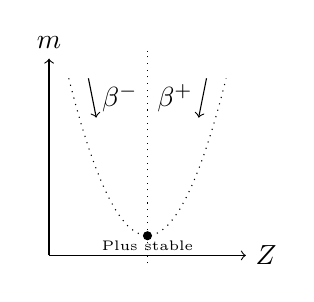
\begin{tikzpicture}[scale=0.5]
                \draw[domain=-2:2, dotted] plot(\x, \x*\x);
                \draw[->] (-2.5, -0.5) -- (-2.5, 4.5);
                \draw[->] (-2.5, -0.5) -- (2.5, -0.5);
                \draw[->] (-1.5,4) -- (-1.3,3);
                \draw[->] (1.5,4) -- (1.3,3);
                \node[above] at (-2.5,4.5) {$m$};
                \node[right] at (2.5,-0.5) {$Z$};
                \node[right] at (-1.4,3.5) {$\beta^-$};
                \node[left] at (1.4,3.5) {$\beta^+$};
                \filldraw (0,0) circle(0.1);
                \node at (0,-0.25) { {\tiny Plus stable}};
                \draw[dotted] (0,-0.7) -- (0,4.7);
            \end{tikzpicture}
            \caption{$A = 121$.}
            \label{06.10.121}
        \end{figure}

    \item \emph{Comment s'exprime le nombre d'anti-neutrinos produit par $^{226}$Ac, selon la diagramme (je ne le peux pas copier)?}

        On commence en notant que $83\%$ des r\'eactions sont la r\'eaction $\beta^-$, qui as un temps charact\'eristique qu'on doit calculer. La demi-vie de $^{226}$Ac est $29$h, et donc la temps charact\'eristiques pour $\beta^-$ est donn\'ee par $\frac{29 \cdot 83\%}{\ln 2}$h. On ne s'inqui\`ete pas des autres r\'eactions parce que seulement $\beta^-$ produit des anti-neutrinos. Donc on a
        \begin{align}
            \rd{N_{\bar{\nu}_e}}{t} &= -\frac{N_{Ac}}{\tau_{\beta^-}}\\
            &= -\frac{N_{Ac}}{\tau_{1/2}}\frac{\ln 2}{0.83}\\
            &\approx \scinot{5.5}{-6}\mathrm{s^{-1}} = 50.4\mathrm{h}
        \end{align}

        Donc on produit $\scinot{5.5}{-6}\mathrm{neutrino/nucleus/s}$. 

        \emph{Comment \'evolue la concentration de $^{226}$Ra en fonction du temps? Si on commence avec un \'echantillion pur de $^{226}$Ac, quelle est la composition chimique \`a $t = 1\mathrm{min}, t = 100 \mathrm{h}, t = 10^4\mathrm{ans}$?}

        L'\'equation qui donne la concentration de $^{226}$Ra est
        \begin{align}
            \rd{^{226}\mathrm{Ra}}{t} &= -\rd{^{226}\mathrm{Ac}}{t}\Bigg|_{\beta^+} + \rd{^{226}\mathrm{Ra}}{t} \Bigg|_{\alpha}
        \end{align}

        Il faut au premier calculer $^{226}\mathrm{Ac}(t) = N_02^{-\frac{t}{\tau_{1/2}}} = N_0e^{-\frac{t}{\tau_{Ac}}}$ et donc ce qu'on veut est
        \begin{align}
            \rd{^{226}\mathrm{Ac}(t)}{t}\Bigg|_{\beta^+} &= \left( 0.17\% \right)\left( -\frac{N_0}{\tau_{Ac}}e^{-\frac{t}{\tau_{Ac}}} \right)\\
            \rd{^{226}\mathrm{Ra}}{t} &= \left( 0.17\% \right)\left( \frac{N_0}{\tau_{Ac}}e^{-\frac{t}{\tau_{Ac}}} \right) - \frac{^{226}\mathrm{Ra}}{\tau_{Ra}}\\
            ^{226}\mathrm{Ra}(t) &= \frac{N_{0}}{\tau_{Ac}/0.17\left( \frac{1}{\tau_{Ac}} - \frac{1}{\tau_{Ra}} \right)} \left[e^{-\frac{t}{\tau_{Ra}}} - e^{-\frac{t}{\tau_{Ac}}}\right]
        \end{align}

        On calcule que $\tau_{Ac} = 43\mathrm{h}, \tau_{Ra} = 2300\mathrm{yr}$ et donc on peut calculer ses trois cas
        \begin{itemize}
            \item $t = 1\mathrm{min}$ --- Les deux exponentielles peuvent \^etre r\'e\'ecrire commes $e^{-\delta} \approx 1 - \delta$ et on obtient $^{226}\mathrm{Ra}(t) \approx \scinot{7}{-5}N_0$. 
            \item $t = 100\mathrm{h}$ --- On a deux cas limites et donc les exponentielles sont essentiellement \'egales \`a $(1 - 0)$ et on obtient $0.17N_0$.
            \item $t = 10^4\mathrm{yr}$ --- On trouve $\scinot{2}{-3}N_0$. 
        \end{itemize}
\end{enumerate}

\section{Age du syst\`eme solaire}

\begin{enumerate}[1.]
    \item \emph{On a $P_i \to F_i$. Trouver $P_i(t), F_i(t)$ en fonction de $P_i(0), F_i(0)$.}

        C'est simplement $P_i(t) = P_i(0)e^{-t/\tau}$, $F_i(t) = F_i(0) + \left( P_i(0) - P_i(t) \right)$.

    \item \emph{Montrer la relation suivante.}
        \begin{align}
            F_1(t) - F_1(0) &= P_1(t)\left( e^{t/\tau_1} - 1 \right)\\
            F_2(t) - F_2(0) &= P_2(t)\left( e^{t/\tau_2} - 1 \right)\\
            \frac{F_1(t) - F_1(0)}{F_2(t) - F_2(0)} &= \frac{P_1(t)\left( e^{t/\tau_1} - 1 \right)}{P_2(t)\left( e^{t/\tau_2} - 1 \right)}
        \end{align}
        et on les divise.
    \item \emph{Pourquoi est-ce que $\alpha(t) = \frac{P_2(t)}{P_1(t)}$ est universelle dans toutes m\'et\'eorites?}

        On assume que $\alpha(0)$ est universelle parce que l'univers primoridial \'etait homog\`ene, et donc $\alpha(t) = \alpha(0)e^{-t\left( \frac{1}{\tau_2} - \frac{1}{\tau_1} \right)}$ et parce qu'on assume $\alpha(0)$ est universelle on sait que $\alpha(t) = 0$ (l'\'exponentielle est naturellement universelle). 
    \item \emph{On trouve que $\alpha(t_0) = \frac{1}{137.9}$ ($t_0$ est la pr\'esente). Si on compare $X_i = \frac{F_i(t)}{S(t)}$ avec $S(t)$ constante, montrer que c'est universelle(?).}

        On note que $\frac{X_2 - \frac{F_2(0)}{S(0)}}{X_1 - \frac{F_1(0)}{S(0)}} = \alpha(t)$ et donc c'est universelle.
\end{enumerate}
\chapter{13/10/14 --- Makeup:Physique Nucl\'eaire, la fusion (en anglais)}

I'm going to do this makeup lecture in English to save some time.

We begin with a description of the cross section classically. Exhibit a particle scattering off a potential $V(r)$, then we want simply the number of particles scattered into the solid angle $\left[ \theta-d\theta, \theta \right]$. The scattering cross section and its differential are given below
\begin{align}
    \frac{d^2N_{scatt}}{dtd\Omega} &= F_m\rd{\sigma_{el}}{\Omega}\\
    \rd{\sigma_{el}}{\Omega} &= \abs{\frac{2\pi b(\theta)db}{2\pi \sin\theta d\theta}}
\end{align}

We can assume classical scattering when the impact parameter is much larger than the characteristic length scale of the incoming paricle, but quantum techniques are necessary when the length scale of the interaction is larger than or of the order of the length scale of the particle's de Broglie wavelength. Theoretical methods for electroweak interactions use perturbative techniques such as the Born approximation while for fusion/nuclear interactions (strong force) we use phenomenological models.

\section{Calculating quantum cross section}

Definition is still the same. We assume initial and final states are plane waves of momentum $p_i, p_f$ scattering off a fixed central potential $V(\abs{\vec{r_1} - \vec{r}_2})$. We throw Fermi's Golden Rule at this and after a bit of math we arrive at the Born approximation
\begin{align}
    \rd{\sigma}{\Omega} &= \frac{E^2}{4\pi^2\left( \hbar c \right)^4}\abs{\tilde{V}(\vec{q})}^2
\end{align}
with $\vec{q} = \vec{p_i} - \vec{p}_f$ and $\tilde{V}$ is the Fourier transform of $V(r)$. We can do a few examples such as Coulomb diffusion (which reproduces the classical result exactly, as one might recall) or the neutrino interaction (weak potential is nearly a delta function).

\section{Thermonuclear fusion}

If we recall the plot of $\frac{B}{A}$ mass per mass number, we find that it increases sharply at first and decays slowly (after iron, recall). Thus, both fusion and fission can be thermodynamically favorable if they are on the right parts of the curve; it is necessary that we fuse lighter elements, to catch the rising part of the curve. Fusion differs from previous calculation because there is no scattering and the nuclear interaction is not a small perturbation. Also, there is no fixed reference frame (products/reagants are usually of comparable size) so we have to go to center of mass frame.

It turns out if we examine the potential carefully we find the Coulomb barrier before the nuclear potential is felt to be far higher than astrophysical conditions! It turns out that we have to tunnel through the barrier. We will walk through the process very roughly.

Let $P = e^{-G}$ be the probability of a state transition, and call $G$ the Gamow factor, then we can find the cross section $\sigma(E) = \frac{S(E)}{E}e^{-G} \propto P$ where the S-factor $S(E)$ takes into account nuclear effects. 

For non-resonant cross sections the $S$ factor is nearly constant, but near resonance like everything else $S(E)$ picks up a Lorentzian shape,
\chapter{03/11/14 --- Fusion dans les \'etoiles}

Pour vaincre la force coulombienne et avoir la fusion nucl\'eaire il faut avoir une \'energie environ $\frac{\alpha \hbar c}{r} \sim 1.4\mathrm{MeV}$. Mais \`a l'int\'erieure du soleil on n'est que $15$ million de degr\'ees, pas suffisaiment chaud pour vaincre la force coulombienne.

On peut calculer la section efficace, qui d\'epend d'un effet de ``tunneling'', et finalement on trouve par quelques calculs qu'il y a un r\'esonance Gamow. Les deux processus de fusion produissent les neutrinos, et on peut les d\'etecter.

La loi de la conservation d'\'energie dit que $\rd{U}{t} = \rd{Q}{t} - P\rd{V}{t}$. Si on l'\'ecrit en terme de la luminosit\'e on trouve que si le soleil evolue lentement la luminosit\'e est \'egale \`a la puissance nucl\'eaire. 

L'\'energie est transport\'ee en trois facon, la radiation, la conduction, et la convection. On sait que la relation entre le flux d'\'energie et la densit\'e d'\'energie \`a une fr\'equence est donn\'ee par $\vec{F}_\nu = -D\nabla u_\nu$. On calcule que par le transport radioactif que $\rd{T}{r} = -\frac{3\overline{\kappa}\rho}{4acT^3}\frac{L(r)}{4\pi r^2}$ ($\kappa$ et l'opacit\'e) la variation de la temperature \`a la distance du centre.

Aussi, on peut calculer la relation entre la masse et la luminosit\'e par la th\'eoreme viriel, et on trouve que $L \propto M^3$, ou plus pr\'ecisement
\begin{align}
    L &= \left(\frac{4\pi}{3}\right)^2\frac{ac}{\kappa}\left(\frac{\beta}{6}\frac{G m_p}{k}\right)^4 M^3
\end{align}

On examine la luminosit\'e d'Eddington et on trouve qu'il y a une luminosit\'e maximum $L_{max} = \frac{4\pi c GM}{\kappa}$. Ca correspond \`a une masse maximum de $M_{max} = 60 N_0m_p = 110 M_\odot$ la masse de Chandresekar. 

Le transport conductif est seulement non-negligible dans un milieu froid et dense, comme un gaz d\'egener\'e. Le transport convectif est aussi pas trop interessant; on examine simplement si un gaz est stable par une action adiabatique.

On a maintenant quatre \'equations de la structure stellaire (pour cinque fonctions $P,M,L,\rho,T$)
\begin{align}
    \rd{P}{r} &= -\rho(r)\frac{GM(r)}{r^2}\\
    \rd{M}{r} &= 4\pi r^2 \rho(r)\\
    \rd{L}{r} &= 4\pi r^2 \rho(\epsilon_{nuc} - \epsilon_\nu)\\
    \rd{T}{r} &= -\frac{3\overline{\kappa}\rho}{4acT^3}\frac{L(r)}{4\pi r^2}
\end{align}
les \'equations de l'equilibre hydrostatique, la conservation de masse, la conservation d'\'energie, et le transfert radiatif. On a besoin d'une \'equation d'\'etat! Le prochain amphi. 

On peut faire une diagramme HR d'un amass des \'etoiles et voir l'\^age de cet amass. 

\chapter{03/11/14 --- PC 6 --- Fusion thermonucl\'eaire}

On finit au d'abord la derni\`ere exercise de la derni\`ere petite classe. Rappelons comme dans la classe on a
\begin{align}
    \expvalue{\sigma v} &\propto \int S(E) e^{-b/\sqrt{E}} e^{-E/kT}\;dE\\
    &\approx S(E_G) \int \exp\left[-\underbrace{\frac{b}{\sqrt{E}} + \frac{E}{kT}}_{\phi(E)}\right]\;dE
\end{align}

On fait l'approximation voyant que $\phi(E)$ est tres \'etroits autour quelque \'energie $E_G$, et on developpe l'\'exponentiel autour le maximum de $\frac{b}{\sqrt{E}} + \frac{E}{kT}$ qui est $E_G = \left(\frac{bkT}{2}\right)^{2/3}$. Maintenant on approxime $e^{-\phi(E)}$ avec un Gaussian, pour qu'il fausse calculer $\Delta$ pour $\phi(E) \simeq \frac{3E_G}{kT} + \frac{(E - E_G)^2}{2\Delta^2}$. On trouve que
\begin{align}
    \Delta &= \sqrt{\frac{2}{3}E_G kT}
\end{align}

Avec ce Gaussian on peut calculer facilement l'int\'egrale si on sait $S(E_G)$, qu'on appelle le facteur de Gamow. C'est pas facile \`a m\'esurer, mais apr\`es une collaboration on sait les $S(E_G)$ pour les $E_G$ solaires.

\section{Fusion thermonucl\`eaire au c\oe ur du soleil}

\begin{enumerate}[1.]
    \item \emph{Donner les r\'eactions les plus simples correspondant \`a la r\'eaction globale 4p $\to$ $^4$He + 2e$^+$ + 2$\nu_E$.}

        \begin{align}
            2(p + p &\to D + e^+ + \nu_e)\\
            2(D + p &\to ^3He + \gamma)\\
            ^3He + ^3He &\to ^4He + 2p
        \end{align}

        Les \'energies liber\'ees dans chaque \'etapes sont faciles \`a calculer par les masses; on trouve qu'elles sont $0.421, 5.495, 12.860$MeV respectivement; en totale $24.69$MeV. Mais parce qu'on est au milieu du soleil, les $e^+$ sont imm\'ediatement \'ecraser comme $e^+ + e^- \to 2\gamma$ et ca produit une nouvelle somme de $26.2$MeV.

    \item \emph{Ecrire les \'equations r\'egissant l'\'evolution des densit\'es des particules $n_p, n_D, n_3, n_4$ les protons, le deut\'erium}
        
        On \'ecrit les relations pour chaque r\'eaction
        \begin{align}
            \dot{R}_1 &= \frac{1}{2}n_pn_p\expvalue{\sigma_{pp} v}\\
            \dot{R}_2 &= n_Dn_p\expvalue{\sigma_{Dp} v}\\
            \dot{R}_3 &= \frac{1}{2}n_3n_3 \expvalue{\sigma_{33} v}
        \end{align}

        Ensuite on sait que
        \begin{align}
            \rd{n_p}{t} &= -2\dot{R}_1 - \dot{R}_2 + 2\dot{R}_3\\
            \rd{n_D}{t} &= \dot{R}_1 - \dot{R}_2\\
            \rd{n_3}{t} &= \dot{R}_2 - 2\dot{R}_3\\
            \rd{n_4}{t} &= \dot{R}_3
        \end{align}
        
        Finalement on assume que $n_D, n_3$ sont constants, parce qu'ils sont des produits interm\'ediates. Ca nous donne que $\dot{R}_1 = \dot{R_2} = 2\dot{R}_3$ et alors $\rd{n_p}{t} = -4\rd{n_4}{t}$. 

        Mais aussi, on voit que $\rd{n_D}{t} = 0$ nous donne $\frac{n_D}{n_p} = \frac{1}{2} \frac{\expvalue{\sigma_{pp}v}}{\expvalue{\sigma_{pD}v}} \sim 10^{-18}$ \`a l'\'equilibre. On voit similairement que $\frac{n_3}{n_p} = \sqrt{\frac{1}{2}\frac{\expvalue{\sigma_{pp}v}}{\expvalue{\sigma_{33} v}}}$. Alors on trouve
        \begin{align}
            \rd{n_p}{t} &= -\expvalue{\sigma_{pp}v}n_p^2
        \end{align}
        et l'\'echelle de temps caracteristique est $\frac{1}{n_p\expvalue{\sigma_{pp}v}}$. 

    \item Ce qui reste c'est de calculer la puissance liber\'ee par le coeur du soleil, et on trouve que c'est \'egale \`a la luminosit\'e, ce qu'on expecte.
\end{enumerate}

\section{Processus $3\alpha$}

Dans les g\'eants on trouve qu'il faut avoir un processus $3\alpha \to ^{12}C$. On l'examine.

\begin{enumerate}[1.]
    \item \emph{Ecrire l'\'evolution des densit\'es num\'eriques des  r\'eactions.}

        Les r\'eactions sont
        \begin{align}
            \alpha + \alpha \rightarrow ^8Be\\
            \alpha + \alpha \leftarrow ^8Be\\
            \alpha + ^8Be \to ^{12} C + \gamma
        \end{align}
        et alors les densit\'es num\'eriques evoluent comme
        \begin{align}
            \rd{n_\alpha}{t} &= -2\dot{R}_1 + 2\dot{R}_2 - \dot{R}_3 &&= -n_\alpha^2\expvalue{\sigma_{\alpha\alpha}v} + 2\frac{n_8}{\tau_8} - n_\alpha n_p \expvalue{\sigma_{\alpha p}v}\\
            \rd{n_8}{t} &=\dot{R}_1 - \dot{R}_2 - \dot{R}_3 &&= \frac{1}{2}n_\alpha^2 \expvalue{\sigma_{\alpha\alpha}v} - \frac{n_8}{\tau_8} - n_\alpha n_8\expvalue{\sigma_{\alpha 8}v}\\
            \rd{n_12}{t} &= \dot{R}_3 &&= n_\alpha n_8 \expvalue{\sigma_{\alpha 8} v}
        \end{align}

    \item Plus tard il faut trouver $\expvalue{\alpha \alpha \alpha}$ qu'on sait est $\rd{n_2}{t}\frac{1}{6}n_\alpha^3\expvalue{\alpha \alpha \alpha}$ et on peut calculer $\rd{n_2}{t}$ par ci-dessus.

\end{enumerate}
\chapter{10/11/14 --- Makeup: Les naines blanches}

Pour d\'ecrire les \'etoiles on a dit qu'on a $4$ \'equations pour $5$ variables. L'\'equation qui nous manque est une \'equation de l'\'etat $P(\rho,T)$. D'abord, il faut d\'efinir la pression, la force raport\'ee \`a l'aire de surface, ou plus pr\'ecisement
\begin{align}
    P &= \frac{1}{3}\int pv(p)n(p)\;dp
\end{align}
ou $p$ est l'impulsion, $v(p)$ est la velocit\'e et $n(p)$ et la densit\'e d'\'etats. Classiquement
\begin{align}
    P &= \frac{1}{3}\int\limits_{0}^{\infty}p\frac{p}{m}\;dp\\
    &= \frac{2}{3} \int E n(p)\;dp = \frac{2}{3}\frac{U}{V}
\end{align}

\section{Un gaz fermionique d\'eg\'ener\'e}

Un tel gaz suit la distribution de Fermi-Dirac
\begin{align}
    n(p) &= 2\frac{4\pi p^2}{\hbar^3}\frac{1}{\exp\left( \frac{E - E_F}{kT} \right) + 1}
\end{align}

Pour un gaz compl\`etement d\'eg\'ener\'e, on trouve ($n(p) = \Theta(p_f - p)$)
\begin{align}
    P &= \frac{1}{3}\int\limits_{0}^{p_F}p\frac{p}{m}\frac{8\pi p^2}{\hbar^3}\;dp\\
    &= \frac{8\pi}{15}\frac{p_F^2}{m}\left( \frac{p_F}{\hbar} \right)^3
\end{align}
ou plus clairement $P \propto n^{5/3}$; la pression est ind\'ependante du temp\'erature.

Si le gaz est relativistique, on trouve que $v(p) = c\frac{p/mc}{\sqrt{1 + (p/mc)^2}}$, et apr\`es des calculs on trouve que $P \propto n^{4/3}$ et qu'elle est \'egalement ind\'ependante du temp\'erature.

Pour un gaz ultrarelativistique, $P = \frac{1}{3}\frac{U}{V}$. On trouve aussi par le th\'eor\`eme du viriel que $3\overline{P}V = -U_G$ et alors $U = -U_G$ qui dit que $E = U + U_G = 0$ l'\'energie total. Alors un gaz ultrarelativistique n'est pas li\'e!

\subsection{Gaz de photons, ou gaz bosonique}

Pour un photon $E = pc, v=c$ et il suit la distribution de Bose-Einstein
\begin{align}
    n(p) &= 2\frac{4\pi p^2}{\hbar^3}\frac{1}{\exp\left( \frac{pc}{kT} \right) - 1}
\end{align}

Alors on calcule que $P = \frac{1}{3}\frac{U}{V} = \frac{1}{3}\frac{8\pi^5}{15}\frac{(kT)^4}{(hc)^3} \equiv a T^4$. 

\section{Les naines blanches}

On note que
\begin{align}
    E_f &= \frac{1}{2m_e}\left( \frac{3\hbar^3n_e}{8\pi} \right)^{2/3}\\
    &\simeq m_e c^2\left( \frac{M}{M_{\odot}} \right)^{4/3}
\end{align}
et donc si la masse augmente, les \'electrons deviennent relativistique!

Il nous faut aussi de noter une autre expression
\begin{align}
    \frac{R}{R_0} &= \left( \frac{M}{M_c} \right)^{1/3}\sqrt{1 - \left( \frac{M}{M_c} \right)^{2/3}}
\end{align}

Ca nous montre que $R \to 0$ lorsque $M \to M_c$. 
\chapter{10/11/14 --- PC 7 --- Supernovae, naines brunes}

\section{Supernovae de Type 1A}

\begin{enumerate}[1.]
    \item \emph{Apr\`es le th\'eor\`eme du viriel, montrer qu'une \'etoile est en \'equilibre stable par rapport d'une \'el\'evation de la temp\'erature centrale $\Delta T > 0$.}

        Rappelons que $3\overline{P}V + E_g = 0 = 2U + E_g, U = \frac{1}{2} E_g \frac{3\overline{P}V}{2}, E = E_g + U = \frac{E_g}{2} = -U$. En \'equilibre stable $\rd{E}{t} = L_{nuc} - L = 0$, $L_{nuc}, L$ les luminosit\'es du noyau et de l'\'etoile respectivement. De plus, $E_g \propto -\frac{GM^2}{R}, U = \frac{3}{2}kTN$ avec $N$ le nombre des particules, ou \'egalement $U \propto MT$.

        Si $\Delta T > 0$ et $\Delta L_{nuc} \gg 0$ (raisonable car $L_{nuc}$ est un exponential sur $T$), alors $L$ augmente apr\`es que la transfert radiatif attendait la surface. On peut calculer ce dur\'ee de temps en le modelant comme une marche al\'eatoire et on le trouve d'\^etre \`a l'ordre de mille ans. Alors car $\rd{E}{t} > 0 \to \rd{U}{t} < 0$, $\rd{T}{t} < 0$ et c'est stable. Aussi, c'est l'\'echelle de cette change qui nous interesse, et on trouve que c'est \`a l'ordre des ondes de son, autrement dit plus vite que $\Delta L$. Alors, une \'etoile est stable par une changement de temp\'erature $\Delta T > 0$. 

    \item \emph{Si une \'etoile compagnon transf\`ere de la mati\`ere sur une naine blache, que se passera-t-il?}

        Une naine blanche est compos\'ee par du gaz d\'eg\'ener\'e, alors $P = k\rho^{5/3}, u = \frac{3}{2}VK\rho^{5/3} \propto  M^{5/3}R^{-2}$. Alors apr\`es le th\'eor\`eme du viriel, $U = \frac{1}{2}E_g \propto \frac{M^2}{R} \propto M^{5/3}R^{-2}$ donc $M^{1/3} \propto R^{-1}$, alors si $M$ augmente $R$ d\'ecro\^it. Aussi, $\rho \propto M^{2}$, donc l'\'etoile devient aussi plus dense. 

    \item \emph{Comparer l'\'energie lib\'er\'ee par la r\'ecation $2^{12}C + 2^{16}O \to ^{56}Ni$ \`a l'\'energie gravitationelle d'une \'etoile.}

        La r\'eaction lib\`ere $44.43$MeV, alors pour une masse du soleil ca lib\`ere \`a l'ordre de $10^{44}$J. L'\'energie gravitationelle lib\`ere \`a l\'ordre de $\frac{GM^2}{R} \sim 10^{43}$J. Alors, si une \'etoile explose par la r\'eaction ci-dessus, 

    \item \emph{Montrer qu'on peut expliquer la luminosit\'e maximum $L_{max} \sim 10^{10}L_{\odot}$.}

        La puissance est $P \propto \rd{N}{t} = -\frac{N}{\tau}$ avec $\tau$ le temps caracter\'eristique $8.8$ jours. Alors on a d\'ej\`a calcul\'e $N$, donc ce n'est pas difficile de calculer $P_{max}$ en utilisant $N_0$ le $N$ au debut de la fusion. C'est $10^{10}L_{\odot}$. 
\end{enumerate}

\section{Naines brunes}

\begin{enumerate}[1.]
    \item \emph{Quel est l'\'echelle de temps $\tau$ de la contraction gravitationelle, appel\`ee \'echelle de temps de Kelvin-Helmholtz?}

        Soit $L$ la luminosit\'e, alors on a encore $\frac{1}{2}E_g = -U, \rd{E}{t} = -L < 0$. Plus pr\'ecisement, $\rd{E}{t} = \rd{}{t}\left( -\alpha \frac{GM^2}{2r} \right) = -L$ et donc $\rd{R}{t} = -\frac{2LR^2}{\alpha GM^2}, \tau = \abs{\frac{1}{R}\rd{R}{t}}^{-1} = \frac{\alpha GM^2}{2RL}$. 

    \item \emph{Aux quelles conditions sur l'\'echelle de temps $t_{KH}$ est l'approximation quasi-statique valable?}

        Car $\tau_{son} \ll \tau_{KH}$, on est toujours \`a l'\'equilibre hydrostatique et on peut utiliser le th\'eor\`eme viriel.

    \item \emph{Que se passe-t-il lorsque $T \gtrsim 10^6$K?}

        Lorsque $T \geq 10^6$K, la fusion commence et une \'etoile est n\'ee. Ca arrive si $R$ d\'ecro\'it.

    \item \emph{Montrque qu'il existe une temp\'erature maximale $T_{max}$ lors de le gaz devient un gaz d\'eg\'ener\'e et pas une \'etoile.}

        Si $T$ devient $<T_{Fermi}$, on aura un gaz d\'eg\'ener\'e et \c{c}a ne produit pas d'\'etoile. On calcule cette condition: la temperature Fermi est
        \begin{align}
            kT_F &= \frac{\left( 3\pi ^2 \hbar^3 n \right)^{2/3}}{2m}
        \end{align}

        Pour l'\'etoile classique, on a $U \propto MT \propto \frac{M^2}{R}$. Le gaz d\'eg\'ener\'e produit $T_F \propto \frac{1}{R^2}$. Donc le seuil de temperature pour que le gaz d\'eg\'ener\'e soit produit existe, car si le temperature baisse trop on atteindra $T_F$ avant $T_{classique}$.

    \item \emph{Comparer la pression radiative et la pression gazeuse pour une \'etoile dans la s\'equence principale.}

        On trouve que $\frac{P_{rad}}{P_{gaz}} = \frac{\frac{1}{3}aT^4}{mkT}$, car $P_{rad} = \frac{1}{3}u$ pour un gaz ultra-relativiste. Alors le rapport est \`a l'ordre de $\propto m^{-1} = \frac{R^3}{M} = M^2$, alors les \'etoiles plus massives ont plus de pression radiative.
\end{enumerate}

\chapter{17/11/14 --- PC 8 --- Neutronisation, Interaction nucl\'eaire dans les \'etoiles \`a neutrons}

\section{Neutronisation}

\begin{enumerate}[1.]
    \item \emph{Montrer que les neutrons apparaissent lorsque la densit\'e atteint $\rho \gtrsim 1,2 \times 10^{7}\mathrm{g/cm^3}$.}

        Les neutrons apparaissent lorsque les \'electrons et les protons combinent, un seuil d'\'en\'energie volum\'etrique qu'on peut calculer apr\`es leurs masses $m_n - m_p - \approx l.293$MeV. Alors si l'\'en\'ergie de l'\'electron est plus que ceci, on trouve les neutrons. Notons que ces \'electrons sont relativistes.

        Apr\`es, il faut trouver la densit\'e correspondant \`a cet \'en\'ergie. La pression est donn\'ee apr\`es $x = \left( 3\pi^2 \right)^{1/3}\left( \frac{\hbar c}{mc^2} \right)n^{1/3}$ par
        \begin{align}
            P &= \frac{1}{24 \pi^2} \frac{(mc^2)^4}{(\hbar c)^3} \times
            \begin{cases}
                \frac{8}{5}x^5 & \mbox{if } x \ll 1\\
                2x^4 & \mbox{if } x \gg 1
            \end{cases}
        \end{align}

        On commence en calculant la quantit\'e de mouvement $E^2 = p^2c^2 + m^2c^4$, alors pour l'\'electron $1.672 = p^2c^2 + 0.261, pc = 1.188$MeV. Alors
        \begin{align}
            \frac{p_Fc}{mc^2}  &= \left( 3\pi^2 \right)^{1/3}\left( \frac{\hbar c}{mc^2} \right)n^{1/3}\\
            1.188 \mathrm{MeV} &= \left( 3\pi^2 \right)^{1/3}\left( 197.327\mathrm{MeV \cdot fm} \right)n^{1/3}\\
            n &= \scinot{7.4}{-9}\mathrm{fm^{-3}}
        \end{align}

        Apr\`es \c{c}a, on calcule $\rho = n\left( m_p + m_e \right) \approx nm_p = 1.258 \times 10^7 \mathrm{g/cm^3}$ car \`a cette densit\'e on n'a que des protons et des \'electrons.

    \item \emph{Ecrire les conditions d'\'equilibre $\beta$. Pour un $n$ on veut trouver la rapport du m\'elange.}

        On essaie maintenant d'\'ecrire l'\'equation d'\'etat. Il faut trouver quelques \'equations
        \begin{align}
            n_e &= n_p\\
            n &= n_e + n_p + n_n
        \end{align}

        La trois\`eme \'equation est donn\'ee par le potentiel chimique pour la r\'eaction $e^- + p^+ \leftrightarrow n^0$. $\mu = E_F$ pour un gaz d\'eg\'ener\'e, et $E_F = \sqrt{(mc^2)^2 + (p_Fc)^2} = (mc^2)\sqrt{1+x^2}$ et alors
        \begin{align}
            m_ec^2\sqrt{1 + x_e^2} + m_pc^2\sqrt{1 + x_p^2} &= m_nc^2\sqrt{1 + x_n^2}\label{17.11.etat}
        \end{align}

        Si on assume la r\'egime ultrarelativiste, $x_e, x_p, x_n \gg 1$, alors l'\'equation ci-dessus devient
        \begin{align}
            m_ex_e + m_px_p &= m_nx_n\\
            n_e^{1/3} + n_p^{1/3} &= n_n^{1/3}\\
            2n_p^{1/3} &= \\
            \frac{n_p}{n_n} &= \frac{1}{8} = \frac{n_e}{n_n}
        \end{align}
        et alors $n_n = 0.8n, n_e = n_p = 0.1n$, mais il faut se rappeler que c'est dans la r\'egime ultrarelativiste.

    \item \emph{On suppose au lieu de la r\'egime ultrarelativiste que $x_e \gg 1, x_p, x_n \ll 1$. Pour quelles densit\'es ces approximations sont-elles valable? Quel est $x_p(x_n)$?}

        C'est facile \`a valider que $x_e \gg 1$ si $\rho \geq \scinot{9.9}{5}$ et que $x_p, x_n \ll 1$ si $\rho \ll \scinot{6}{15}$. On commence on \'ecrivant $x_em_e = x_pm_p$ car $n_e = n_p$. Alors l'\'equation \eqref{17.11.etat} devient
        \begin{align}
            m_e\sqrt{1 + \frac{m_p^2}{m_e^2}x_p^2} + m_p\sqrt{1 + x_p^2} &= m_n\sqrt{1 + x_n^2}\\
            m_px_p + m_p\left( 1 + \frac{x_p^2}{2} \right) &\approx m_n\left( 1 + \frac{x_n^2}{2} \right)\\
            m_p\left( 1 + x_p \right) + O(x_p^2) &\approx m_n\left( 1 + \frac{x_n^2}{2} \right)\\
            x_p &\approx \frac{m_n - m_p}{m_p} + \frac{1}{2}\frac{m_n}{m_p}x_n^2
        \end{align}

        Si $x_n \ll 1$ on ne peut pas n\'egliger $m_n - m_p$.

    \item \emph{A quelle $\rho$ est-ce que la pression des neutrons devient dominante?}

        On note que $P_e > P_p$ toujours, alors il faut simplement comparer $P_e, P_n$. Pour les neutrons qui sont non-relativiste, $P_n = \frac{1}{15\pi^2}\frac{(m_nc^2)^4}{(\hbar c)^3}x_n^5$ et pour les \'electrons ultra-relativiste $P_e = \frac{1}{12\pi^2}\frac{(m_ec^2)^4}{(\hbar c)^3}x_e^4$. La condition que $P_n \gg P_e$ et \'egalement $(m_ex_e)^4 = (m_px_p)^4 \ll \frac{4}{5}m_n^4x_n^5$. Alors au seuil du dominance de $P_n$ on trouve que
        \begin{align}
            \left( \frac{4}{5} \right)^{\frac{1}{4}}\frac{m_n}{m_p}x_n^{5/4} \approx \frac{m_n - m_p}{m_p} + \frac{1}{2} \frac{m_n}{m_p}x_n^2
        \end{align}

        On suppose que $x_n^2$ est la terme la plus petite (car $x_n \ll 1$) et on obtient
        \begin{align}
            \left( \frac{4}{5} \right)^{1/4}\frac{m_n}{m_p}x_n^{5/4} &\approx \frac{m_n - m_p}{m_p}\\
            x_n &\approx \left( \frac{m_n - m_p}{m_n}\left( \frac{5}{4} \right)^{1/4} \right)^{4/5} \approx \scinot{5}{-3}\\
            x_p &\approx \frac{m_n - m_p}{m_p} \approx \scinot{1}{-3}\\
            x_e &\approx \frac{m_n - m_p}{m_e} \approx 2.6\\
            n_n &= \scinot{6}{32}\mathrm{cm^{-3}}\\
            n_p &= \scinot{1}{31}\mathrm{cm^{-3}}\\
            n_e &= \scinot{1}{31}\mathrm{cm^{-3}}\\
            \rho &= n_nm_n + n_pm_p + n_em_e \approx n_nm_n\\
            &= \scinot{9}{8}\mathrm{g\cdot cm^{-3}}
        \end{align}
\end{enumerate}

\section{Interaction nucl\'eaire dans les \'etoiles \`a neutrons}

\begin{enumerate}[1.]
    \item \emph{Calculer le rayon d'une \'etoile \`a neutron et une naine blanche pour $M \sim M_{\odot}$.}

        Commen\c{c}ons par le th\'eor\`eme du viriel $3PV + E_g = 0$, alors $P = -\frac{E_g}{3V} = \frac{\alpha}{4\pi}\frac{GM^2}{R^4}$. La pression est donn\'ee $P = \frac{K}{m}n^{5/3}$ pour un gaz non-relativiste.
        
        On consid\`ere d'abord l'\'etoile \`a neutron, o\`u $n_n = \frac{e}{m_n} = \frac{3M}{4\pi R^3 m_n}$, et pour une naine blanche $n_e = Z\frac{e}{Am_b} = \frac{Z}{A}\frac{3M}{4\pi R^3 m_b}$. Le rapport peut donc \^etre calculer et car on sait que le rayon pour la naine blanche est $10^{-2}R_{\odot}$, on peut calculer le rayon de cette \'etoile, et c'est \`a l'ordre de $10\mathrm{km}$!

        Pour une \'etoile \`a neutrons, $\frac{GM}{Rc^2} \approx 0.2$ alors il faut utiliser les calcules du relativit\'e g\'en\'erale. Pour une naine blanche, ce quantit\`e est $\sim 10^{-3}$ et pour le soleil $\sim10^{-6}$. 
\end{enumerate}
\chapter{24/11/14 --- PC 9 --- Statistique nucl\'eaire}

La densit\'e des particules en g\'en\'eral (relativiste) est donn\'ee par
\begin{align}
    \rd{n}{p} &= \frac{4\pi g}{\hbar^3}\frac{p^2}{\exp\left( \frac{E-\mu}{kT} \right) \pm 1}
\end{align}
o\`u $E^2 = p^2c^2 + m^2c^4$. Pour les bosons, $g=2$ et on utilise $-$ dans le d\'enominateur, et les Fermions $g=2s+1, +$. Par exemple, pour les photons $\mu = 0, E = pc$ et on trouve toutes les relations normales. Pour les fermions en g\'en\'eral, il faut considerer dans quelle r\'egime nous sommes. Relativiste vs. non-relativiste, $pc \gtrless mc^2$, d\'eg\'ener\'e vs. non-d\'eg\'ener\'e, $kT \gtrless \mu$. Par exemple, les fermions non-relativistes non-d\'eg\'ener\'es on trouve la distribution de Maxwell-Boltzmann
\begin{align}
    \rd{n}{E} &= \frac{gm^{3/2}}{\sqrt{2}\pi^2\hbar^3}\left( E-mc^2 \right)^{1/2}e^{-\frac{E - \mu}{kT}}
\end{align}

On peut calculer les densit\'es, les \'en\'energies et les pressions alors. Pour les fermions d\'eg\'ener\'es, $kT \gg E - \mu$, et alors la distribution devient un fonction en escalier $\Theta(E-\mu)$. 

\section{Equilibre statistique nucl\'eaire}

\begin{enumerate}[1.]
    \item \emph{A l'\'equilibre de la r\'eaction $n,p \leftrightarrow (A,Z) + \gamma$ quels sont les fractions de masse en fonction de l'\'energie de liason du noyau?}

        La r\'eaction $n,p \leftrightarrow (A,z) + \gamma$ est en \'equilibre si et seulement si les potentiels chimiques sont \'egales, qui est
        \begin{align}
            (A-Z)\mu_n + Z\mu_p = \mu_A
        \end{align}

        On le remplace dans la distribution de Fermi-Dirac pour les $n_A$, o\`u $B_A$ est l\'energie de liason
        \begin{align}
            n_A &= g_A\left( \frac{m_A kT}{2\pi \hbar^2} \right)^{\frac{3}{2}}\exp\left( \frac{(A-Z)(\mu_n - m_nc^2) + Z(\mu_p - m_pc^2) + B_A}{kT} \right)\\
            &= n_n^{(A-Z)}n_p^{Z}\frac{g_A}{2^{A}} \left( \frac{m_A}{m_n^{A-Z}m_p^{Z}} \right)^{\frac{3}{2}}\left( \frac{ kT}{2\pi \hbar^2} \right)^{\frac{3}{2}\left( 1 - A \right)}e^{\frac{B_A}{kT}}
        \end{align}
        o\`u $g_p = g_n = \frac{1}{2}$. D'ici c'est facile d'obtenir les fractions de masse selon les $n_A, n_p, n_n$. 

        On trouve que pour les atomes gros, $n_a \propto T^{-A + 1}$ alors \c{c}a change beaucoup avec la temperature. C'est car les photons photo-dissocie les atomes.

    \item \emph{Analyser un diagramme.}

        Pour verifier qu'on est non-relativiste, on compare l'\'energie cin\'etique \`a $mc^2$, et pour verifier qu'on est non-d\'eg\'ener\'e on compare $kT_F$ \`a la temp\'erature du gaz.
\end{enumerate}

\section{Nucl\'eosynth\`ese primordiale}

En fonction de la temperature, les \'elements plus lourd qui ont l'\'energie de liason la plus petite pour un rapport particulier des concentrations des protons et des neutrons dominent les temperatures froides, les protons/neutrons dominent les temperatures chaudes (car tout est dissoci\'e), et He$^4$ domine dans les temperatures interm\'ediates car il est l'atome de l\'energie de liason la plus haute de tous atomes l\'eger.

L'\'echelle dynamique du temps est donn\'ee par $t_{dyn} = \abs{\frac{1}{T}\rd{T}{t}}^{-1}$, et car $T \propto t^{-\frac{1}{2}}$ on trouve que $t_{dyn} = 2t = 360 \mathrm{s} T^{-2}$. 




\emph{A quelle temperature commence la r\'eaction $p + n \leftrightarrow D + \gamma$?}

On commence avec $\tau = \abs{\frac{1}{n_p}\rd{n_p}{t}}^{-1}$ o\`u $n_p$ peut \^etre n'importe lequel de $p,n$, et $\tau' = \abs{\frac{1}{n_D}\rd{n_D}{t}}^{-1}$ la dissociation. Alors la r\'eaction commence si $\tau > \tau'$. On peut calculer les temps caracteristiques comme
\begin{align}
    \rd{n_p}{t} &= -n_pn_n \expvalue{\sigma v}_{pn}
\end{align}
etc.
\end{document}
